In the appendices of~\autoref{chap:subgraph_counting} and~\autoref{chap:antipattern}, and~\textsection~\autoref{antipattern:sec:termination_criterion}, we present some propositions, lemmas, and theorems.
The dependency structure among these results is clarified in~\autoref{fig:dependency_graph}.
\begin{figure}
\resizebox{0.9\textwidth}{!}{

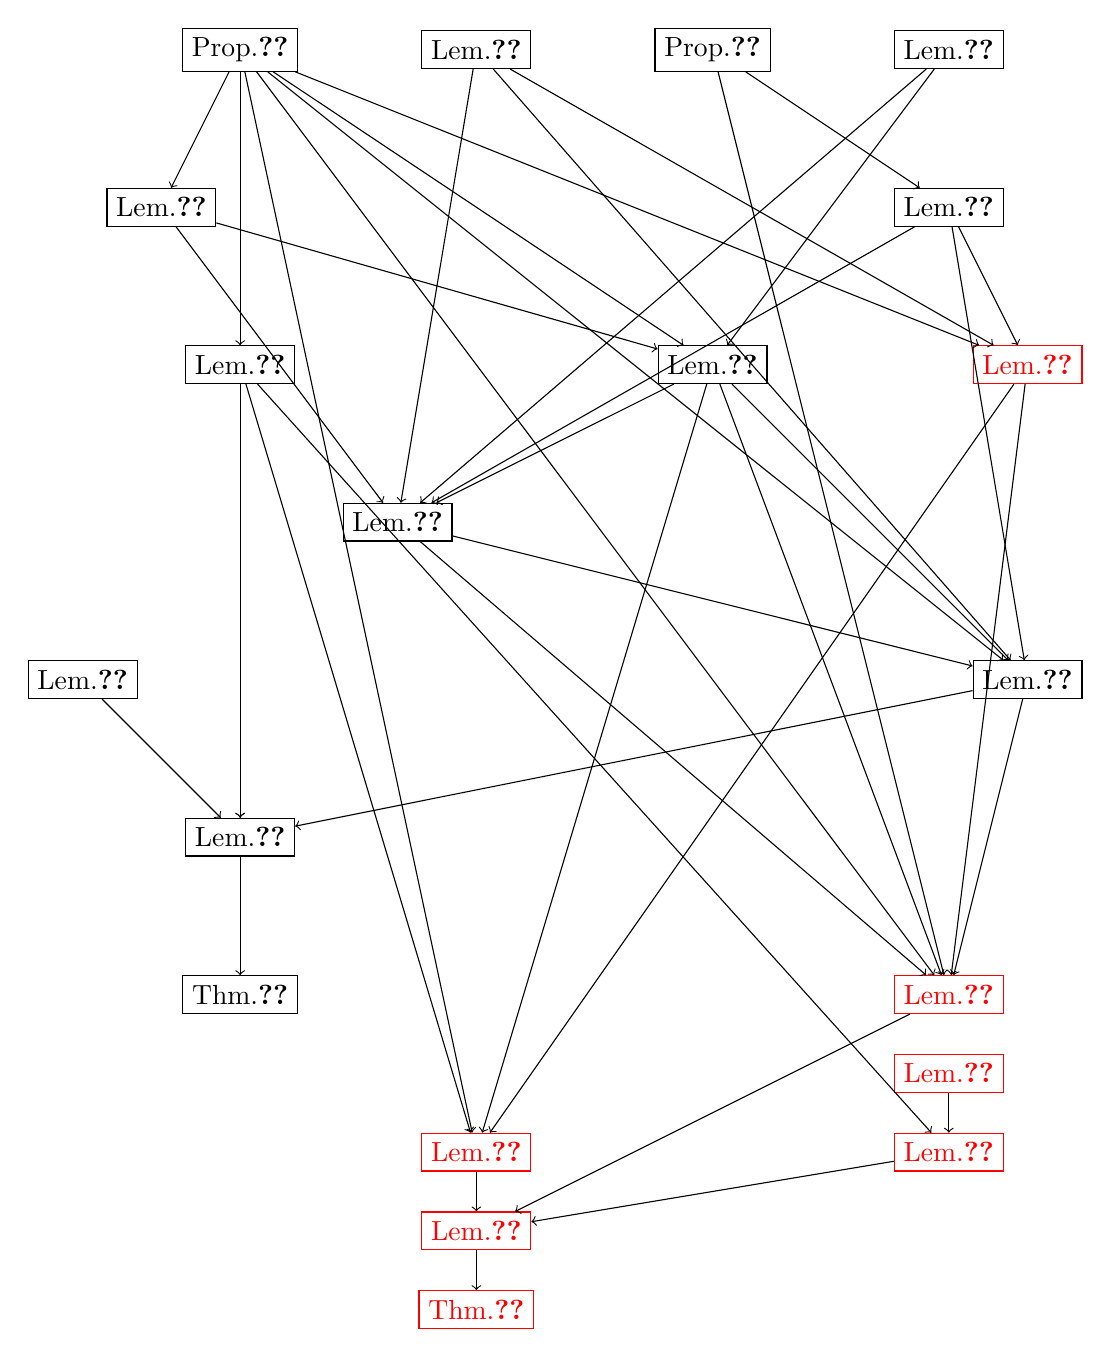
\begin{tikzpicture}

    \node[draw] (prop_pb_eq_po) at (0,12) {Prop.$\ref{prop:pb_eq_po}$};
    \node[draw] (kpcpck_pullback) at (3,12) {Lem.$\ref{kpcpck_pullback}$};
    \node[draw] (prop_graph_adhesive) at (6,12) {Prop.$\ref{prop:graph_adhesive}$};
  \node[draw] (lem_xinXcpinCrpinR) at (9,12) {Lem.$\ref{lem:xinXcpinCrpinR}$};

    \node[draw] (lem_b_c_same_img_exist_a) at (-1,10) {Lem.$\ref{lem:b_c_same_img_exist_a}$};
    \node[draw] (kpcpxrp_po) at (9,10) {Lem.$\ref{kpcpxrp_po}$};
    
    \node[draw] (subgraph_counting_lem_decomp_w_u) at (0,8) {Lem.$\ref{subgraph_counting:lem:decomp_w_u}$};
    \node[draw] (lem_g_monic) at (6,8) {Lem.$\ref{lem:g_monic}$};

   \node[draw] (lem_h_hp_diff_g_gp_diff) at (2,6) {Lem.$\ref{lem:h_hp_diff_g_gp_diff}$};
  

    \node[draw] (subgraph_counting_lem_xlnlmxrnr) at (-2,4) {Lem.$\ref{subgraph_counting:lem:xlnlmxrnr}$};
    \node[draw] (subgraph_counting_lem_w_u_l_not_geq_r_not) at (10,4) {Lem.$\ref{subgraph_counting:lem:w_u_l_not_geq_r_not}$};

    \node[draw] (subgraph_counting_lem_w_g_geq_w_h_leq) at (0,2) {Lem.$\ref{subgraph_counting:lem:w_g_geq_w_h_leq}$};
    \node[draw,red] (antipattern_lem_xgm_xhmp_xl_xr_llsss) at (9,-1) {Lem.$\ref{antipattern:lem:xgm_xhmp_xl_xr_llsss}$};
    \node[draw,red] (antipattern_lem_xh_decomp) at (10,8) {Lem.$\ref{antipattern:lem:xh_decomp}$};

    \node[draw](subgraph_counting_thm_termination_grs) at (0,0) {Thm.$\ref{subgraph_counting:thm:termination_grs}$};

    \node[draw,red] (antipattern_lem_xgm_xhmp_xl_xr) at (9, -2) {Lem.$\ref{antipattern:lem:xgm_xhmp_xl_xr}$};

        \draw[->] (prop_pb_eq_po) to (lem_b_c_same_img_exist_a);
        \draw[->] (prop_graph_adhesive) to (kpcpxrp_po);
        \draw[->] (lem_xinXcpinCrpinR) to  (lem_g_monic);
        \draw[->] (lem_b_c_same_img_exist_a) -- (lem_g_monic);
        \draw[->] (prop_pb_eq_po) to (lem_g_monic);
        
        \draw[->] (kpcpck_pullback) to (lem_h_hp_diff_g_gp_diff);
        \draw[->] (kpcpxrp_po) to  (lem_h_hp_diff_g_gp_diff);
        \draw[->] (lem_g_monic) to  (lem_h_hp_diff_g_gp_diff);
        \draw[->] (lem_xinXcpinCrpinR) -- (lem_h_hp_diff_g_gp_diff);
        \draw[->] (lem_b_c_same_img_exist_a) to (lem_h_hp_diff_g_gp_diff);

        \draw[->] (prop_pb_eq_po) to (subgraph_counting_lem_decomp_w_u);

        \draw[->] (prop_pb_eq_po)to  (subgraph_counting_lem_w_u_l_not_geq_r_not);
        \draw[->] (kpcpck_pullback) to (subgraph_counting_lem_w_u_l_not_geq_r_not);
        \draw[->] (kpcpxrp_po) to (subgraph_counting_lem_w_u_l_not_geq_r_not);
        \draw[->] (lem_g_monic) to (subgraph_counting_lem_w_u_l_not_geq_r_not);
        \draw[->] (lem_h_hp_diff_g_gp_diff) to (subgraph_counting_lem_w_u_l_not_geq_r_not);

        \draw[->] (subgraph_counting_lem_decomp_w_u) to  (subgraph_counting_lem_w_g_geq_w_h_leq);
        \draw[->] (subgraph_counting_lem_decomp_w_u) to (subgraph_counting_lem_w_g_geq_w_h_leq);
        \draw[->] (subgraph_counting_lem_w_u_l_not_geq_r_not) to (subgraph_counting_lem_w_g_geq_w_h_leq);
        \draw[->] (subgraph_counting_lem_xlnlmxrnr) to (subgraph_counting_lem_w_g_geq_w_h_leq);

        \draw[->] (subgraph_counting_lem_w_g_geq_w_h_leq) to (subgraph_counting_thm_termination_grs);

        \draw[->] (subgraph_counting_lem_decomp_w_u) to (antipattern_lem_xgm_xhmp_xl_xr);
        \draw[->] (antipattern_lem_xgm_xhmp_xl_xr_llsss) to (antipattern_lem_xgm_xhmp_xl_xr);


        % \draw[->] (prop_pb_eq_po) to (antipattern_lem_xh_decomp);
        % \draw[->] (kpcpck_pullback) to (antipattern_lem_xh_decomp);
        % \draw[->] (kpcpxrp_po) to (antipattern_lem_xh_decomp);

        \draw[->] (prop_pb_eq_po) to (antipattern_lem_xh_decomp);
        \draw[->] (kpcpck_pullback) to (antipattern_lem_xh_decomp);
        \draw[->] (kpcpxrp_po) to (antipattern_lem_xh_decomp);

        \node[draw,red] (antipattern_lem_xglnotmlp_xhlnotmrp) at (3,-2) {Lem.$\ref{antipattern:lem:xglnotmlp_xhlnotmrp}$};
        % \draw[->] (subgraph_counting_lem_w_u_l_not_geq_r_not) to (antipattern_lem_xglnotmlp_xhlnotmrp);
        \draw[->] (prop_pb_eq_po) to (antipattern_lem_xglnotmlp_xhlnotmrp);
        \draw[->] (subgraph_counting_lem_decomp_w_u) to (antipattern_lem_xglnotmlp_xhlnotmrp);
        \draw[->] (antipattern_lem_xh_decomp) to (antipattern_lem_xglnotmlp_xhlnotmrp);
        \draw[->] (lem_g_monic) to (antipattern_lem_xglnotmlp_xhlnotmrp);
        % \draw[->] (lem_h_hp_diff_g_gp_diff) to (antipattern_lem_xglnotmlp_xhlnotmrp);
        % \draw[->] (prop_graph_adhesive) to (antipattern_lem_xglnotmlp_xhlnotmrp);

        \node[draw,red] (antipattern_lem_xglnotmlnotlp_xhlnotmrnotrp) at (9, 0) {Lem.$\ref{antipattern:lem:xglnotmlnotlp_xhlnotmrnotrp}$};
        \draw[->] (subgraph_counting_lem_w_u_l_not_geq_r_not) to (antipattern_lem_xglnotmlnotlp_xhlnotmrnotrp);
        \draw[->] (lem_g_monic) to (antipattern_lem_xglnotmlnotlp_xhlnotmrnotrp);
        \draw[->] (antipattern_lem_xh_decomp) to (antipattern_lem_xglnotmlnotlp_xhlnotmrnotrp);

        \draw[->] (lem_h_hp_diff_g_gp_diff) to (antipattern_lem_xglnotmlnotlp_xhlnotmrnotrp);

        \draw[->] (prop_graph_adhesive) to (antipattern_lem_xglnotmlnotlp_xhlnotmrnotrp);
        \draw[->] (prop_pb_eq_po) to (antipattern_lem_xglnotmlnotlp_xhlnotmrnotrp);
        
        \node[draw,red] (antipattern_lem_w_g_geq_w_h_leq) at (3,-3) {Lem.$\ref{antipattern:lem:w_g_geq_w_h_leq}$};
        \draw[->] (antipattern_lem_xglnotmlp_xhlnotmrp) to (antipattern_lem_w_g_geq_w_h_leq);
        \draw[->] (antipattern_lem_xglnotmlnotlp_xhlnotmrnotrp) to (antipattern_lem_w_g_geq_w_h_leq);
        \draw[->] (antipattern_lem_xgm_xhmp_xl_xr) to (antipattern_lem_w_g_geq_w_h_leq);

        \node[draw,red] (antipattern_thm_termination_grs) at (3,-4) {Thm.$\ref{antipattern:thm:termination_grs}$};
        \draw[->] (antipattern_lem_w_g_geq_w_h_leq) to  (antipattern_thm_termination_grs);
    \end{tikzpicture} 
}
    \caption{Dependency graph}
    \label{fig:dependency_graph}
\end{figure}
